\section{Результаты}

В эксперименте использовались две установки соответственно двум методам определения скорости звука. Первая установка состояла из раздвижной трубы с миллиметровой шкалой. Труба наполнялась воздухом через патрубок. Вторая установка содержала теплоизолированную трубу фиксированных размеров, помещённую в термостат. Более подробное описание экспериментальных установок см. в \nameref{Приложение 1}.

Для наблюдения резонанса, возникавшего в трубе, использовался цифровой осциллограф. Резонанс характеризовался увеличением амплитуды колебаний сигнала на осциллографе.

Частота звуковой волны устанавливалась с помощью звукового генератора.

Температура $T$ воздуха в трубе устанавливалась с помощью контроллера термостата. Газ, текущий через трубу, обменивался энергией с водой внутри термостата и нагревался до нужной температуры.

По измеренным зависимостям $(L_{n+k} - L_n)(k)$ (результаты в таблицах 1,2,3,4,5 см. \nameref{Приложение 2}) для пяти различных частот $f$ звуковой волны построены графики. Результаты представлены на рисунке рис. 1.

\begin{figure} [h]
    \label{figure1}
    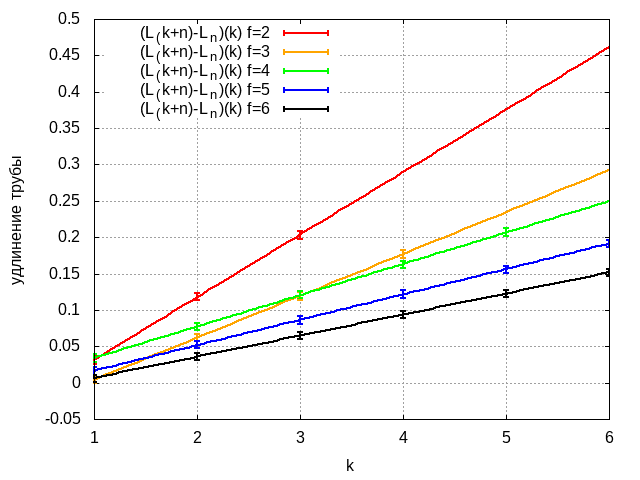
\includegraphics[width=0.9\textwidth]{img/graph9.png}

    \caption{Графики зависимости удлинения трубы от номера резонанса $k$ при различных частотах звуковой волны.}
    
\end{figure}

По методу наименьших квадратов определены коэффициенты $\alpha$ наклона прямых. Затем по \eqref{eq: L_nk} и \eqref{eq: c} определена скорость звука при каждой частоте звуковой волны. 

\begin{table}[h]
    \centering
    \begin{tabular}{|c|c|c|c|c|c|c|c|}
    \hline
    $\alpha, \text{м}$ & $f\cdot 10^{3}, \text{Гц}$ & $\lambda, \text{м}$ & $c, \frac{\text{м}}{\text{с}}$ & $\sigma_\alpha \cdot 10^{-3}, \text{м}$ & $\sigma_f, \text{Гц}$ & $\sigma_\lambda \cdot 10^{-3}, \text{м}$ & $\sigma_c, \frac{\text{м}}{\text{с}}$ \\ \hline
    0.086   & 2 & 0.172 & 344 & 0.58 & 3 & 1.16 & 2.34\\ \hline
    0.058   & 3 & 0.116 & 348 & 0.14 & 3 & 0.28 & 0.91\\ \hline
    0.043   & 4 & 0.086 & 344 & 0.30 & 3 & 0.60 & 2.41\\ \hline
    0.035   & 5 & 0.070 & 350 & 0.14 & 3 & 0.28 & 1.42\\ \hline
    0.029   & 6 & 0.058 & 348 & 0.14 & 3 & 0.28 & 1.69\\ \hline
\end{tabular}
    \caption{Зависимость скорости $c$ звука в воздухе от частоты $f$ звуковой волны. $\alpha$ - угловой коэффициент графика зависимости $(L_{n+k} - L_n)(k)$, $\lambda$ - длина волны, $\sigma_\alpha, \sigma_f, \sigma_\lambda, \sigma_c$ - погрешности измерения углового коэффициента, частоты, длины волны, скорости звука соответственно.}
    \label{tab:t10}
\end{table}
\newpage
Из таблицы 1 следует, что скорость звука в воздухе не зависит от частоты звуковой волны в представленном диапазоне частот. Передача колебаний молекул осуществляется через упругие соударения, и этот процесс не зависит от частоты колебаний (при частотах в диапазоне от $20\text{Гц}$ до $100 \text{КГц}$).

Среднее значение скорости звука, вычисленное по таблице 1 составляет
\[ c = (346.8 \pm 1.8) \frac{\text{м}}{\text{с}}\]


По измеренным зависимостям $(f_{k+1} - f_1)(k)$ (результаты в таблицах 6,7,8,9,10 см. \nameref{Приложение 3}) для пяти различных температур $T$ воздуха построены графики. Результаты представлены на рисунке рис. 2.

\begin{figure} [h]
    \label{figure4}
    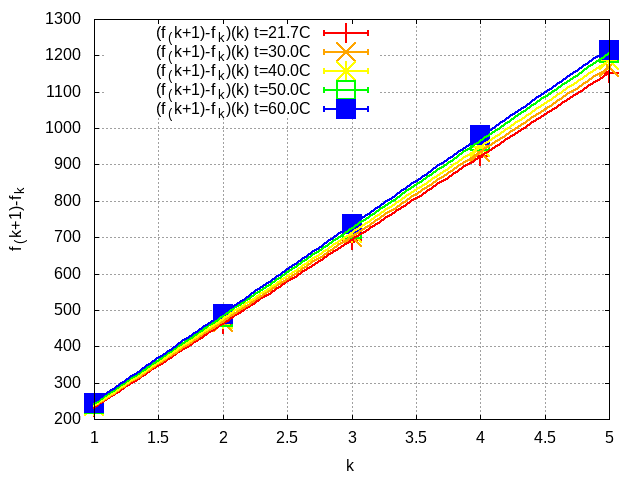
\includegraphics[width=0.9\textwidth]{img/graph8.png}

    \caption{Графики зависимости разности $f_{k+1} - f_1$ частоты текущего и первого резонансов от номера резонанса $k$ при различных температурах $T$ воздуха.}
    
\end{figure}
\newpage
Графики являются линейными, что согласуется с теорией (выражение \eqref{eq: fk}). При увеличении температуры воздуха угловой коэффициент графиков увеличивается, и из этого следует, что увеличивается скорость звука (выражение \eqref{eq: fk}). Это подтверждается тем, что при увеличении температуры газа увеличивается кинетическая энергия молекул газа, значит, повышается интенсивность их взаимодействия.

По методу наименьших квадратов определены коэффициенты $\beta$ наклона прямых. Затем по \eqref{eq: fk} определена скорость звука при каждой температуре воздуха. Результаты приведены в таблице 2.

\begin{table}[h]
    \centering
    \begin{tabular}{|c|c|c|c|c|c|c|}
    \hline
    $\beta, \text{c}^{-1}$ & $T, \celsius$ & $L, \text{м}$ & $c, \frac{\text{м}}{\text{с}}$ & $\sigma_\beta, \text{c}^{-1}$ & $\sigma_L\cdot 10^{-3}, \text{м}$ & $\sigma_c, \frac{\text{м}}{\text{с}}$ \\ \hline
    230.2   & 21.7 & 0.74 & 340.7 & 0.28 & 1 & 0.6 \\ \hline
    233.3   & 30.0 & 0.74 & 345.3 & 0.25 & 1 & 0.6 \\ \hline
    237.2   & 40.0 & 0.74 & 351.1 & 0.40 & 1 & 0.8 \\ \hline
    241.2   & 50.0 & 0.74 & 357.0 & 0.31 & 1 & 0.7 \\ \hline
    243.2   & 60.0 & 0.74 & 360.0 & 1.19 & 1 & 0.9 \\ \hline
\end{tabular}
    \caption{Зависимость скорости $c$ звука в воздухе от температуры $T$ воздуха. $\beta$ - угловой коэффициент графика зависимости $(f_{k+1} - f_1)(k)$, $L$ - длина трубы, $\sigma_\beta, \sigma_L, \sigma_c$ - погрешности измерения углового коэффициента, длины трубы, скорости звука соответственно.}
    \label{tab:t10}
\end{table}

Использованы значения величин из таблицы 2, чтобы определить показатель адиабаты воздуха при различных температурах. Результаты приведены в таблице 3.

\begin{table}[h]
    \centering
    \begin{tabular}{|c|c|c|c|c|c|}
    \hline
    $c, \frac{\text{м}}{\text{с}}$ & $T, \celsius$ & $\gamma$ & $\sigma_c, \frac{\text{м}}{\text{с}}$ &  $\sigma_T, \celsius$ & $\sigma_\gamma\cdot 10^{-3}$ \\ \hline
    340.7   & 21.7 & 1.370 & 0.6 & 0.1 & 4.86 \\ \hline
    345.3   & 30.0 & 1.373 & 0.6 & 0.1 & 4.79 \\ \hline
    351.1   & 40.0 & 1.374 & 0.8 & 0.1 & 6.28 \\ \hline
    357.0   & 50.0 & 1.377 & 0.7 & 0.1 & 5.42 \\ \hline
    360.0   & 60.0 & 1.358 & 0.9 & 0.1 & 6.80 \\ \hline
\end{tabular}
    \caption{Зависимость показателя адиабаты $\gamma$ воздуха от температуры $T$ воздуха. $c$ - скорость звука в воздухе, $\sigma_c, \sigma_T, \sigma_\gamma$ - погрешности измерения скорости звука, температуры воздуха, показателя адиабаты соответственно.}
    \label{tab:t10}
\end{table}

Из таблицы 3 следует, что показатель адиабаты $\gamma$ постоянен в исследованном диапазоне температур газа. $\gamma$ зависит от количества активированных степеней свободы газа. При температурах воздуха, приведенных в работе, у газа активированы только вращательные и поступательные степени свободы, и энергии молекул недостаточно, чтобы активировать колебательные.

Через \eqref{eq: i} определено количество степеней свободы воздуха в предположении, что воздух считается идеальным газом.
\[ i \approx 5\]
Значит, воздух является двухатомным газом с 5 степенями свободы: 3 - поступательные, 2 - вращательные.
